\documentclass{thesis}

\title{硒化镉量子点的二维光谱探测}
\author{陈稼霖} % 学生姓名
\id{45875852} % 学号
\entranceYear{2017} % 入学年份
\institute{物质科学与技术学院} % 院系名称
\major{物理学} % 二级学科专业名称
\advisor{John A. McGuire} % 指导教师:姓名
\date{二零二一~年~六~月} % 毕业日期:夏季为6月、冬季为12月

\titleEn{Two-dimensional Spectroscopy of \text{CdSe} Quantum Dots}% Title
\authorEn{Jialin Chen}% Student name
\instituteEn{School of Physical Science and Technology}% 院系名称
\majorEn{Physics}% 二级学科专业名称
\advisorEn{John A. McGuire}% Advisor
\dateEn{June / 2021}% 毕业日期:夏季为June、冬季为December

\begin{document}
\frontmatter
\maketitle
\maketitleEn
\makedeclaration
\makeabstract{% 中文摘要
    二维光谱是一种基于三阶非线性光学效应的超快时间分辨的光谱测量手段。它用三个激光脉冲组成的序列激励材料,得到以泵浦和探测频率为自变量的非线性光学响应谱。相较传统一维光谱,二维光谱能够揭示材料更为丰富的信息:其对角峰反映了材料的能级分布,而非对角峰则反映了能级间的耦合关系。本项目以硒化镉量子点这一具有分立能级且研究得较为透彻的材料为样品,利用二维电子光谱研究的其电子动力学机制。我们首先利用紫外可见吸收光谱获得了硒化镉量子点的能级分布的大致情况,然后通过瞬态吸收谱确定了产生单激子激发的泵浦能量范围,在确保单激子激发的前提下,我们测量了硒化镉量子点的二维光谱,并对二维光谱进行了初步的分析。
}{% 中文关键词
    硒化镉量子点,瞬态吸收,二维光谱
}
\makeenglishabstract{% English abstract
    Two-dimensional spectroscopy is an ultrafast laser spectroscopy technology based on third order nonlinear effect. It excites the material with sequences of three laser pulses, and obtains a non-linear optical response spectrum with pump and probe frequencies as variables. Compared with traditional one-dimensional spectroscopy, two-dimensional spectroscopy can reveal richer information of materials: its diagonal peaks reflect the energy level distribution of the materials, while non-diagonal peaks reflect the coupling relationship between the energy levels. This project takes cadmium selenide quantum dots, a material that has discrete energy levels and has been studied thoroughly, as sample, and uses two-dimensional electronic spectroscopy to study its electronic dynamics mechanism. We first obtained the general situation of the energy level distribution of the cadmium selenide quantum dots with ultraviolet-visible absorption spectrum, and then determined the pump energy range for single-exciton regime by measuring transient absorption. In single exciton regime, We measured the two-dimensional spectrum of cadmium selenide quantum dots and make some simple analysis.
}{% English key words
    Two-dimensional spectroscopy, transient absorption, CdSe quantum dots.
}
\begin{spacing}{1}
    \zihao{5}\tableofcontents
    \thispagestyle{empty}
\end{spacing}
\mainmatter
\chapter{背景介绍}
\thispagestyle{firstpagestyle}

\section{量子点}
纳米晶体(nanocrystals)是尺寸在百纳米以下的晶体颗粒。尺寸在纳米级别的纳米晶体又称量子点(quantum dots)。一颗量子点的尺寸与数百至数十个晶格周期的长度相当,其中包含有数百万到数千个原子。纳米晶体是一种准零维的材料,其中的电子的波函数受到三个正交方向上的约束,类似于处于一个三维势阱中的粒子的波函数,故有别于传统体块材料的连续能带,量子点表现出分立的能级。材料量子点的空穴态(electron states)和电子态(hole states),与体块材料中的价带和导带相对应,在 $0$ K 下分别处于完全被电子占据和完全不被电子占据的状态。相对于体块材料的带隙,量子点电子态的最高能级和空穴态的最低能级之差更大,可由布鲁斯公式(Brus Equation)\cite{brus1986electronic}\cite{kippeny2002semiconductor}估算,
\begin{align}
    \label{Brus Equ}
    \Delta E\approx E_{\text{gap}}+\frac{h^2}{8r^2}\left(\frac{1}{m_e^*}+\frac{1}{m_h^*}\right)-\frac{1.8e^2}{4\pi\epsilon_0\epsilon_rr},
\end{align}
其中 $E_{\text{gap}}$ 为对应体块材料的带隙,$r$ 为量子点的半径,$m_e^*$ 和 $m_h^*$ 为材料中电子和空穴的有效质量,$e$ 为元电荷大小,$\epsilon_0$ 为真空中介电常数,$\epsilon_r$ 为材料的介电常数。

\subsection{硒化镉量子点的能级结构}
硒化镉(cadmium selenide,化学式 \ce{CdSe})量子点,有闪锌矿型(zinc blende,图 \ref{CdSe Quantum Dot} (a))和纤锌矿型(wurtzite,图 \ref{2D Spectrum System} (b))两种类型的结构,前者属于立方晶系(图 \ref{CdSe Quantum Dot} (c)),后者属于六方晶系(图 \ref{CdSe Quantum Dot} (d))。两种晶体结构具有基本相同的能级结构,仅在晶格势(来自于六方晶系的非对称性)和电子-空穴交换相互作用导致的能级劈裂表现上略有差异 \cite{efros1996band},但在本实验的分辨率下这些差异并不显著。\ce{CdSe} 量子点的具体能级如图 \ref{CdSe Quantum Dot} (e) 所示,允许的激子激发过程按能级差从小到大排列为 1S$_{3/2}\rightarrow$1S(e) 跃迁, 1P$_{3/2}\rightarrow$1S(e) 跃迁, 1P$_{3/2}\rightarrow$1S(e) 跃迁和 2S$_{1/2}\rightarrow$1S(e)跃迁。从激子的角度来看,\ce{CdSe} 量子点的能级等价于图 \ref{CdSe Quantum Dot} (f) 所示的激子能级结构,基态为 $\lvert 0\rangle$,四种跃迁产生的激子态分别为 $\lvert 1\rangle$, $\lvert 2\rangle$, $\lvert 3\rangle$ 和 $\lvert 4\rangle$。

\begin{figure}[h]
    \centering
    \includegraphics[width=.8\columnwidth]{CdSe Quantum Dot.pdf}
    \caption{(a)(b) 闪锌矿型和纤锌矿型 \ce{CdSe} 晶体结构;(c)(d) 闪锌矿型和纤锌矿型 \ce{CdSe} 晶体结构 $c$ 方向视图;(e) \ce{CdSe} 量子点的电子态和空穴态能级(改自 \cite{caram2014persistent}),纵向箭头代表允许的激子激发过程;(f) \ce{CdSe} 量子点的激子能级(改自 \cite{caram2014persistent})。}
    \label{CdSe Quantum Dot}
\end{figure}

\section{二维光谱}
二维光谱是一种基于三阶非线性光学效应的超快时间分辨的光谱测量手段。图 \ref{2D Spectrum Intro}(a) 展示了二维光谱的一般构型,三个光脉冲依次以一定的角度入射待测样品,在某一方向上对信号光进行探测。为方便起见,前两个脉冲称为泵浦脉冲,而后一个脉冲称为探测脉冲。通过扫描脉冲的中心频率,和/或扫描脉冲间的时延并关于时延做傅里叶变换,可以得到信号光强度关于泵浦频率和探测频率的光谱,此即二维光谱。

\begin{figure}[h]
    \centering
    \includegraphics[width=.8\columnwidth]{Img/2D Spectrum Intro.pdf}
    \caption{(a) 一个典型的二维光谱构型:三个光脉冲分别经一凸透镜聚焦,分别由 $\bm{k}_1$, $\bm{k}_2$, $\bm{k}_3$ 方向入射样品,在 $\bm{k}_3+\bm{k}_2-\bm{k}_1$ 方向上探测信号光。(b) 本实验采用的二维光谱构型:两个泵浦脉冲由同一方向入射样品,而后探测脉冲由另一方向入射样品,并在探测脉冲方向上进行探测。(c) 两个激子的部分能级(横向黑色实线)间的耦合以及允许的跃迁过程(纵向箭头),其中 $E_{nm}$ 代表两个激子分别处于 $\lvert m\rangle$ 态和 $\lvert n\rangle$ 态时对应的能级,黑色箭头代表泵浦过程,灰色箭头代表探测过程。(d) 子图 (c) 中各允许的跃迁过程在二维光谱中对应的信号峰,其中黑色代表负响应(漂白和受激发射),灰色代表正响应(受激吸收)。(改自 \cite{hamm2011concepts} Figure 1.5)}
    \label{2D Spectrum Intro}
\end{figure}

二维光谱可以反映半导体中的激子能级分布及其之间的耦合。激子的耦合类似于类氢原子结合形成分子,一个激子产生的局部电场会使另一激子的激发频率发生斯塔克频移(Stark shift),从而使整体的能量降低。在量子点中,由于激子被束缚在较小的空间中,因此激子间的耦合作用较强。图 \ref{2D Spectrum Intro} 展示了两个激子的部分能级间的耦合情况,耦合的 $\lvert m\rangle$ 态和 $\lvert n\rangle$ 态的激子的能量要稍低于单独激发 $\lvert m\rangle$ 态和 $\lvert n\rangle$ 态激子的能量之和。图 \ref{2D Spectrum Intro}(c) 和 (d) 展示了二维光谱中涉及的跃迁过程和二维光谱中信号峰的对应关系。在单激子激发(single-exciton regime)的情形下,扫描泵浦和探测脉冲的频率。当泵浦脉冲的频率与 $\lvert 1\rangle$ 态激子的激发频率共振,则发生图 \ref{2D Spectrum Intro}(c) 中标号为 \textcircled{\footnotesize{1}} 的受激吸收,产生一个 $\lvert 1\rangle$ 态的激子,随后的探测脉冲可以再激发另一 $\lvert 1\rangle$ 态或 $\lvert 2\rangle$ 态的激子(图 \ref{2D Spectrum Intro}(c) 中标号分别为 \textcircled{\footnotesize{5}} 和 \textcircled{\footnotesize{6}}),在图 \ref{2D Spectrum Intro}(d) 中显示为正响应的信号峰,由于系统在基态的布居数的减少,图 \ref{2D Spectrum Intro}(c) 中标号为 \textcircled{\footnotesize{1}} 和 \textcircled{\footnotesize{3}} 的受激吸收减弱,在图 \ref{2D Spectrum Intro}(d) 中表现为负响应的信号峰,此外,图中 \ref{2D Spectrum Intro}(c) 中标号为 \textcircled{\footnotesize{2}} 的受激辐射也贡献了图 \ref{2D Spectrum Intro}(d) 中负响应的对角信号峰。当泵浦脉冲的频率与 $\lvert 2\rangle$ 的激子的激发频率共振时探测光产生的跃迁过程,可以同理对应到图 \ref{2D Spectrum Intro} 中的信号峰。

在我们的实验中,如图 \ref{2D Spectrum Intro}(b),两个泵浦脉冲以 $\bm{k}_1$ 的方向入射样品,探测脉冲以 $\bm{k}_2$ 的方向入射样品。两个泵浦脉冲分别带有相位 $\phi_1$ 和 $\phi_2$,两个泵浦脉冲之间的时延为 $\tau$,后一个泵浦脉冲和探测脉冲之间的时延为 $T$。入射的两个泵浦脉冲和探测脉冲的电场分量可以分别表示为
\begin{align}
    \notag\bm{E}_{\text{pump},1}(t)=&2\mathcal{E}_1(t+\tau)\cos[\omega_1(t+\tau)-\bm{k}_1\cdot\bm{r}+\phi_1]\hat{e}\\
    =&\mathcal{E}_1(t+\tau)\left\{e^{i[\omega_1(t+\tau)-\bm{k}_1\cdot\bm{r}+\phi_1]}+e^{-i[\omega_1(t+\tau)-\bm{k}_1\cdot\bm{r}+\phi_1]}\right\}\hat{e},\\
    \notag\bm{E}_{\text{pump},2}(t)=&\bm{E}_{\text{pump},1}(t-\tau)=2\mathcal{E}_1(t)\cos[\omega_1t-\bm{k}_1\cdot\bm{r}+\phi_2]\hat{e}\\
    =&\mathcal{E}_1(t)\left\{e^{i[\omega_1t-\bm{k}_1\cdot\bm{r}+\phi_2]}+e^{-i[\omega_1t-\bm{k}_1\cdot\bm{r}+\phi_2]}\right\}\hat{e},\\
    \notag\bm{E}_{\text{probe}}(t)=&2\mathcal{E}_2(t-T)\cos[\omega_2(t-T)-\bm{k}_2\cdot\bm{r}]\hat{e}\\
    =&\mathcal{E}_2(t-T)\left\{e^{i[\omega_2(t-T)-\bm{k}_2\cdot\bm{r}]}+e^{-i[\omega_2(t-T)-\bm{k}_2\cdot\bm{r}]}\right\}\hat{e},
\end{align}
其中$\mathcal{E}_1(t)$ 和 $\mathcal{E}_2(t)$ 分别为泵浦光和探测光脉冲的包络函数,两者均仅在 $t=0$ 附近不为零,$\omega_1$ 和 $\omega_2$ 分别为泵浦光和探测光的(中心)频率,$\bm{k}_1$ 和 $\bm{k}_2$ 分别为泵浦光和探测光的波矢量。
总光场的电场强度为以上三束光的电场强度的矢量叠加,
\begin{align}
    \bm{E}_{\text{tot}}(t)=\bm{E}_1(t)+\bm{E}_2(t)+\bm{E}_3(t).
\end{align}
简单起见,认为诱导产生的电偶极矩方向与电场方向平行,总光场与量子点之间的电偶极相互作用哈密顿量为
\begin{align}
    \hat{H}_{I,\text{tot}}(t)=-\hat{\bm{p}}\cdot\bm{E}_{\text{tot}}(t)=\sum_{m\neq n}p_{mn}E_{\text{tot}}(t)\lvert m\rangle\langle n\rvert=\hat{H}_I(t)+H_I^{\dagger}(t),
\end{align}
其中量子点的电偶极矩
\begin{align}
    \hat{\bm{p}}=\sum_{m\neq n}p_{mn}\lvert m\rangle\langle n\rvert.
\end{align}

时域上,在上述相互作用哈密顿量的扰动下,故密度矩阵的三阶微扰修正项为(详见附录 \ref{von Neumann Equ sol})
\begin{align}
    \rho^{(3)}(t)=\hat{U}_0(t)\left(-\frac{i}{\hbar}\right)^3\int_{\tau_0}^t\mathrm{d}\tau_3\int_{\tau_0}^{\tau_3}\mathrm{d}\tau_2\int_{\tau_0}^{\tau_2}\mathrm{d}\tau_1\,\left[\hat{H}_I'(\tau_3),\left[\hat{H}_I'(\tau_2),\left[\hat{H}_I'(\tau_1),\hat{\rho}^{(0)}(\tau_0)\right]\right]\right]\hat{U}_0(-t),
\end{align}
其中初始状态下,系统的绝大多数布居集中于基态,密度矩阵可以近似表示为
\begin{align}
    \hat{\rho}^{(0)}(t=0)=\lvert 0\rangle\langle 0\rvert,
\end{align}
$\hat{H}_I'(t)$ 为 $\hat{H}_I(t)$ 在相互作用绘景中的形式。
密度矩阵的修正项中含有 $e^{\pm i\bm{k}_2\cdot\bm{r}}$ 相位的相干矩阵元才对 $\bm{k}_2$ 方向的信号光有所影响,因此我们只需考虑修正项的这一部分
\begin{align}
    \notag\rho^{(3)}(t)=\hat{U}_0(t)\left(-\frac{i}{\hbar}\right)^3\int_{\tau_0}^t\mathrm{d}\tau_3\int_{\tau_0}^{\tau_3}\mathrm{d}\tau_2\int_{\tau_0}^{\tau_2}\mathrm{d}\tau_1\,&\left[\hat{H}_I'(\tau_3)\hat{H}_I'^*(\tau_2)\hat{H}_I'(\tau_1)\hat{\rho}^{(0)}(\tau_0)\right.\\
    \notag&+\hat{H}_I'(\tau_1)\hat{\rho}^{0}(\tau_0)\hat{H}_I'^*(\tau_2)\hat{H}_I'(\tau_3)\\
    \notag&+\hat{H}_I'(\tau_2)\hat{\rho}^{(0)}(\tau_0)\hat{H}_I'^*(\tau_1)\hat{H}_I'(\tau_3)\\
    &\left.+\hat{H}_I'(\tau_3)\hat{\rho}^{(0)}(\tau_0)\hat{H}_I'^*(\tau_1)\hat{H}_I'(\tau_2)\right]\hat{U}_0(-t)+\text{h.c.},
    % \notag=&\left(-\frac{i}{\hbar}\right)^3\int_{\tau_0}^t\mathrm{d}\tau_3\int_{\tau_0}^{\tau_3}\mathrm{d}\tau_2\int_{\tau_0}^{\tau_2}\mathrm{d}\tau_1\times\\
    % \notag&\left[\hat{U}_0(t-\tau_3)\hat{H}_I(\tau_3)\hat{U}_0(\tau_3-\tau_2)\hat{H}_I^*(\tau_2)\hat{U}_0(\tau_2-\tau_1)\hat{H}_I(\tau_1)\hat{U}_0(\tau_1)\hat{\rho}^{(0)}(\tau_0)\hat{U}_0(-\tau_1)\hat{U}_0(-(\tau_2-\tau_1))\hat{U}_0(-(\tau_3-\tau_2))\hat{U}_0(-(t-\tau_3))\right.\\
    % \notag&+\hat{U}_0(t-\tau_3)\hat{U}_0(\tau_3-\tau_2)\hat{U}_0(\tau_2-\tau_1)\hat{H}_I(\tau_1)\hat{U}_0(\tau_1)\hat{\rho}^{(0)}(\tau_0)\hat{U}_0(-\tau_1)\hat{U}_0(-(\tau_2-\tau_1))\hat{H}_I^*(\tau_2)\hat{U}_0(-(\tau_3-\tau_2))\hat{H}_I(\tau_3)\hat{U}_0(-(t-\tau_3))\\
    % \notag&+\hat{U}_0(t-\tau_3)\hat{U}_0(\tau_3-\tau_2)\hat{H}_I(\tau_2)\hat{U}_0(\tau_2-\tau_1)\hat{U}_0(\tau_1)\hat{\rho}^{(0)}(\tau_0)\hat{U}_0(-\tau_1)\hat{H}_I(\tau_1)\hat{U}_0(-(\tau_2-\tau_1))\hat{U}_0(-(\tau_3-\tau_2))\hat{H}_I(\tau_3)\hat{U}_0(-(t-\tau_3))\\
    % &\left.+\hat{U}_0(t-\tau_3)\hat{U}_0(\tau_3-\tau_2)\hat{H}_I(\tau_3)\hat{U}_0(\tau_2-\tau_1)\hat{U}_0(\tau_1)\hat{\rho}^{(0)}(\tau_0)\hat{U}_0(-\tau_1)\hat{H}_I^*(\tau_1)\hat{U}_0(-(\tau_2-\tau_1))\hat{H}_I(\tau_2)\hat{U}_0(-(\tau_3-\tau_2))\hat{U}_0(-(t-\tau_3))\right]+\text{h.c.},
\end{align}
其中 h.c. 表示厄米共轭。图 \ref{Feynman Diagram} 展示了产生以上密度矩阵修正项的过程对应的费曼图。
\begin{figure}[h]
    \centering
    \includegraphics[width=.5\columnwidth]{Img/Feynman Diagram.pdf}
    \caption{含 $e^{-i\bm{k}_2\cdot\bm{r}}$ 相位的密度矩阵三阶微扰修正项对应的费曼图。简单起见,仅考虑了单个激子的能级,没有考虑多激子耦合的能级。}
    \label{Feynman Diagram}
\end{figure}
由于 $\mathcal{E}_1(t)$ 和 $\mathcal{E}_2(t)$ 仅在 $t=0$ 附近不等于零,故有近似
\begin{align}
    \int_{\tau_0}^{\tau_2}\mathrm{d}\tau_1\,\hat{H}_I(\tau_1)\approx&e^{i(-\bm{k}_1\cdot\bm{r}-\phi_1)}\int_{-\tau-\Delta\tau}^{-\tau+\Delta\tau}\mathrm{d}\tau_1\,\mathcal{E}_1(\tau_1),\\
    \int_{\tau_0}^{\tau_3}\mathrm{d}\tau_2\,\hat{H}_I(\tau_2)\approx&e^{i(-\bm{k}_1\cdot\bm{r}+\phi_2)}\int_{-\Delta\tau}^{+\Delta\tau}\mathrm{d}\tau_2\,\mathcal{E}_1(\tau_2),\\
    \int_{\tau_0}^t\mathrm{d}\tau_3\hat{H}_I(\tau_3)\approx&e^{-i\bm{k}_3\cdot\bm{r}}\int_{T-\Delta T}^{T+\Delta T}\mathrm{d}\tau_3\,\mathcal{E}_2(\tau_3).
\end{align}
从而将该三阶微扰修正项写为
{\small
\begin{align}
    \label{Density matrix-Time domain-3rd order corrrection}
    \notag\hat{\rho}^{(3)}(t)\approx&\left(-\frac{i}{\hbar}\right)^3\times\\
    \notag&\left[\sum_{n\neq 0}p_{n0}p_{10}^2e^{-i\Omega_{n0}(t-T)-i\Omega_{00}T-i\Omega_{10}\tau+i(\phi_1-\phi_2)}\lvert n\rangle\langle 0\rvert+p_{10}^3e^{-i\Omega_{10}(t-T)-i\Omega_{11}T-i\Omega_{10}\tau+i(\phi_1-\phi_2)}\lvert n\rangle\langle 0\rvert\right.\\
    \notag&\left.+p_{10}^3e^{-i\Omega_{10}(t-T)-i\Omega_{11}T-i\Omega_{01}\tau-i(\phi_1-\phi_2)}\lvert 1\rangle\langle 0\rvert+\sum_{n\neq 0}p_{n0}p_{10}^2e^{-i\Omega_{n0}(t-T)-i\Omega_{00}T-i\Omega_{01}\tau-i(\phi_1-\phi_2)}\lvert n\rangle\langle 0\rvert\right]\times\\
    &\int_{-\Delta T}^{+\Delta T}\mathcal{E}_2(\tau_3)\,\mathrm{d}\tau_3\left(\int_{-\Delta\tau}^{\Delta\tau}\mathcal{E}_1(\tau_1)\,\mathrm{d}\tau_1\right)^2e^{-i\bm{k}_2\cdot\bm{r}}+\text{h.c.}.
\end{align}
}%
这里取“$\approx$”是因为通过旋波近似(rotation wave approximation,简称 RWA)略去了非共振项,其中 $\Omega_{mn}$ 的实部为能级间的共振频率,虚部为能级间的退相干系数,刻画了系统密度矩阵由高能级向低能级弛豫(均匀退相干)的速率,
\begin{align}
    \Omega_{mn}=&\omega_{mn}-i\Gamma_{mn},\\
    \omega_{mn}=&E_{mn}/\hbar,\\
    \Gamma_{mn}=&\Gamma_{nm},
\end{align}
$E_{mn}$ 为能级 $\lvert m\rangle$ 与 $\lvert n\rangle$ 间的能量差。

该三阶微扰项产生的电极化强度为
\begin{align}
    \langle\bm{P}^{(3)}(t)\rangle=\tr\left[N\hat{\bm{p}}\hat{\rho}^{(3)}(t)\right].
\end{align}
其中 $N$ 为粒子数密度。
该电极化强度对 $\bm{k}_2$ 方向的信号有两方面的影响。一方面,极化的样品对探测光存在吸收作用。探测光感受到的样品的电极化率为
\begin{align}
    \chi^{(3)}=\frac{P^{(3)}}{E_{\text{probe}}}.
\end{align}
而探测光在非磁性样品(相对磁导率 $\mu_r=0$)中的衰减系数为
\begin{align}
    \alpha=\im\left[\sqrt{\varepsilon_r\mu_r}\right]=\im\left[\sqrt{\varepsilon_r}\right]=\im\left[\sqrt{1+\chi^{(3)}}\right]\approx\frac{1}{2}\im\left[\chi^{(3)}\right].
\end{align}
另一方面,随时间变化的电极化强度向外辐射电磁波,
\begin{align}
    E_{\text{sig}}\propto\ddot{P}^{(3)}(t).
\end{align}
样品中各个粒子由于自己及其所处环境(如量子点的大小、量子点运动造成的多普勒效应、局部的电磁场、量子点间的相互作用等)的微小差异,导致其能级略有差异,即各粒子的 $\omega_{mn}$ 并非完全相等,而是存在一个分布 $g(\{\omega_{mn}\})$($\{\omega_{mn}\}$ 是包含各个能级共振频率的集合),这导致了系统的非均匀退相干。考虑到这一点,系统的密度矩阵应写为
{\small
\begin{align}
    \label{Density matrix-Time domain-3rd order corrrection-2}
    \notag\hat{\rho}^{(3)}(t)\approx&\left(-\frac{i}{\hbar}\right)^3\int\prod_{m<n}\mathrm{d}\omega_{mn}\,g(\{\omega_{mn}\})\times\\
    \notag&\left[\sum_{n\neq 0}p_{n0}p_{10}^2e^{-i\Omega_{n0}(t-T)-i\Omega_{11}T-i\Omega_{10}\tau+i(\phi_1-\phi_2)}\lvert n\rangle\langle 0\rvert+p_{10}^3e^{-i\Omega_{10}(t-T)-i\Omega_{11}T-i\Omega_{10}\tau+i(\phi_1-\phi_2)}\lvert n\rangle\langle 0\rvert\right.\\
    \notag&\left.+p_{10}^3e^{-i\Omega_{10}(t-T)-i\Omega_{11}T-i\Omega_{01}\tau-i(\phi_1-\phi_2)}\lvert 1\rangle\langle 0\rvert+\sum_{n\neq 0}p_{n0}p_{10}^2e^{-i\Omega_{n0}(t-T)-i\Omega_{00}T-i\Omega_{01}\tau-i(\phi_1-\phi_2)}\lvert n\rangle\langle 0\rvert\right]\times\\
    &\int_{-\Delta T}^{+\Delta T}\mathcal{E}_2(\tau_3)\,\mathrm{d}\tau_3\left(\int_{-\Delta\tau}^{\Delta\tau}\mathcal{E}_1(\tau_1)\,\mathrm{d}\tau_1\right)^2e^{-i\bm{k}_2\cdot\bm{r}}+\text{h.c.}.
\end{align}
}
上式的中括号内第一、二项在均匀退相干效应和非均匀退相干的共同作用下随着时间衰减,而第三、四项在 $(-\tau,0)$ 时间间隔内的非均匀退相干可以被 $T$ 时刻之后的非均匀退相干抵消,故产生信号光的强度在探测光照射后先随时间衰减,后在 $T+\tau$ 时刻重新增强到一极大值,这是一种类似自旋回波(spin echo)的光子回波(photon echo)效应。在我们的实验中,由于缺少对脉冲色散的补偿,脉冲在时域上的宽度较大,光子回波的效应并不显著,信号的强度主要受样品对探测光吸收的影响。

我们还可以从频域上看二维光谱的过程,从而更好地解释二维光谱信号峰的位置。在频域上,两个泵浦光脉冲和探测光脉冲可以表示为
\begin{align}
    \tilde{\bm{E}}_{\text{pump},1}(\bm{r},\omega)=&\left[\tilde{\mathcal{E}}_1(\omega-\omega_1)e^{i(-\bm{k}_1\cdot\bm{r}+\phi_1)}+\tilde{\mathcal{E}}_1(\omega+\omega_1)e^{-i(-\bm{k}_1\cdot\bm{r}-\phi_1)}\right]e^{i\omega\tau}\hat{e}\\
    \tilde{\bm{E}}_{\text{pump},2}(\bm{r},\omega)=&\tilde{\mathcal{E}}_1(\omega-\omega_1)e^{i(\bm{k}_1\cdot\bm{r}-\phi_2)}+\tilde{\mathcal{E}}_1(\omega+\omega_1)e^{i(-\bm{k}_1\cdot\bm{r}-\phi_2)}\hat{e},\\
    \bm{E}_{\text{probe}}(\bm{r},\omega)=&\left[\tilde{\mathcal{E}}_2(\omega-\omega_2)e^{-i\bm{k}_2\cdot\bm{r}}+\tilde{\mathcal{E}}_2(\omega+\omega_2)e^{i\bm{k}_2\cdot\bm{r}}\right]e^{-i\omega T}\hat{e},
\end{align}
其中 $\tilde{\mathcal{E}}_1(\omega)$ 和 $\tilde{\mathcal{E}}_1(\omega)$ 分别为泵浦光脉冲和探测光脉冲包络函数 $\mathcal{E}_1(t)$ 和 $\mathcal{E}_2(t)$ 的傅里叶变换,
\begin{align}
    \tilde{\mathcal{E}}_1(\omega)=&\frac{1}{2\pi}\int_{-\infty}^{+\infty}\mathcal{E}_1(\tau')e^{-i\omega\tau'}\,\mathrm{d}\tau',\\
    \tilde{\mathcal{E}}_2(\omega)=&\frac{1}{2\pi}\int_{-\infty}^{+\infty}\mathcal{E}_2(\tau')e^{-i\omega\tau'}\,\mathrm{d}\tau',
\end{align}
带有 $e^{\pm i\bm{k}_2\cdot\bm{r}}$ 相位的密度矩阵三阶修正项为
\begin{align}
    \notag\hat{\rho}^{(3)}(\omega)\approx&\left[\sum_{n\neq 0}\frac{p_{n0}p_{10}^2\tilde{\mathcal{E}}_1(\omega_{10}-\omega_1)\tilde{\mathcal{E}}_1(\omega_{01}+\omega_1)\tilde{\mathcal{E}}_2(\omega-\omega_2)e^{i[\omega_{10}\tau+(\phi_1-\phi_2)]}}{\hbar^3(\omega_{10}-\Omega_{10})(-\Omega_{00})(\omega-\Omega_{n0})}\right.\\
    \notag&+\frac{p_{10}^3\tilde{\mathcal{E}}_1(\omega_{10}-\omega_1)\tilde{\mathcal{E}}_1(-\omega_{10}+\omega_1)\tilde{\mathcal{E}}_2(\omega-\omega_2)e^{i[\omega_{10}\tau+(\phi_1-\phi_2)]}}{\hbar^3(\omega_{10}-\Omega_{10})(-\Omega_{11})(\omega-\Omega_{10})}\\
    \notag&+\frac{p_{10}^3\tilde{\mathcal{E}}_1(-\omega_{10}+\omega_1)\tilde{\mathcal{E}}_1(\omega_{10}-\omega_1)\tilde{\mathcal{E}}_2(\omega-\omega_2)e^{-i[\omega_{10}\tau+(\phi_1-\phi_2)]}}{\hbar^3(-\omega_{10}-\Omega_{01})(-\Omega_{11})(\omega-\Omega_{10})}\\
    \notag&\left.+\sum_{n\neq 0}\frac{p_{n0}p_{10}^2\tilde{\mathcal{E}}_1(-\omega_{10}+\omega_1)\tilde{\mathcal{E}}_1(\omega_{10}-\omega_1)\tilde{\mathcal{E}}_2(\omega-\omega_2)e^{-i[\omega_{10}\tau+(\phi_1-\phi_2)]}}{\hbar^3(-\omega_{10}-\Omega_{01})(-\Omega_{00})(\omega-\Omega_{n0})}\right]e^{i\omega\tau}e^{-i\omega T}e^{-i\bm{k}_2\cdot\bm{r}}\\
    &+\text{h.c.}.
\end{align}
扫描两个泵浦光之间的时间间隔 $\tau$,并对其做傅里叶变换可得
{\small
\begin{align}
    \notag\hat{\rho}^{(3)}(\omega_{\tau},\omega)=&\left[\sum_{n\neq 0}\frac{p_{n0}p_{10}^2\tilde{\mathcal{E}}_1(\omega_{10}-\omega_1)\tilde{\mathcal{E}}_1(\omega_{01}+\omega_1)\tilde{\mathcal{E}}_2(\omega-\omega_2)\delta(\omega_{\tau}-\omega_{10})e^{i(\phi_1-\phi_2)}}{\hbar^3(\omega_{10}-\Omega_{10})(-\Omega_{00})(\omega-\Omega_{n0})}\lvert n\rangle\langle 0\rvert\right.\\
    \notag&+\frac{p_{10}^3\tilde{\mathcal{E}}_1(\omega_{10}-\omega_1)\tilde{\mathcal{E}}_1(-\omega_{10}+\omega_1)\tilde{\mathcal{E}}_2(\omega-\omega_2)\delta(\omega_{\tau}-\omega_{10})e^{i(\phi_1-\phi_2)}}{\hbar^3(\omega_{10}-\Omega_{10})(-\Omega_{11})(\omega-\Omega_{10})}\lvert 1\rangle\langle 0\rvert\\
    \notag&+\frac{p_{10}^3\tilde{\mathcal{E}}_1(-\omega_{10}+\omega_1)\tilde{\mathcal{E}}_1(\omega_{10}-\omega_1)\tilde{\mathcal{E}}_2(\omega-\omega_2)\delta(\omega_{\tau}+\omega_{10})e^{-i(\phi_1-\phi_2)}}{\hbar^3(-\omega_{10}-\Omega_{01})(-\Omega_{11})(\omega-\Omega_{10})}\lvert 1\rangle\langle 0\rvert\\
    \notag&\left.+\sum_{n\neq 0}\frac{p_{n0}p_{10}^2\tilde{\mathcal{E}}_1(-\omega_{10}+\omega_1)\tilde{\mathcal{E}}_1(\omega_{10}-\omega_1)\tilde{\mathcal{E}}_2(\omega-\omega_2)\delta(\omega_{\tau}+\omega_{10})e^{-i(\phi_1-\phi_2)}}{\hbar^3(-\omega_{10}-\Omega_{01})(-\Omega_{00})(\omega-\Omega_{n0})}\lvert n\rangle\langle 0\rvert\right]e^{-i\omega T}e^{-i\bm{k}_2\cdot\bm{r}}\\
    &+\text{h.c.}.
\end{align}
}%
因此二维光谱中,在泵浦频率和探测频率分别与允许的能级跃迁频率共振处会存在信号峰。

\section{瞬态吸收}
实际实验中得到的二维光谱信号中还含有瞬态吸收信号,在费曼图中对应于一个泵浦脉冲与系统发生两次相互作用,而另一脉冲未与系统发生相互作用的过程(图 \ref{Feynman Diagram-Transient Absorption})。
\begin{figure}[h]
    \centering
    \includegraphics[width=.5\columnwidth]{Img/Feynman Diagram-Transient Absorption.pdf}
    \caption{瞬态吸收过程对应的费曼图。}
    \label{Feynman Diagram-Transient Absorption}
\end{figure}

与这些瞬态吸收过程对应的密度矩阵的三阶微扰修正项为
\begin{align}
    \notag\hat{\rho}^{(3)}(\omega)=&\left[\frac{p_{10}^3\tilde{\mathcal{E}}_1(\omega_{10}-\omega_1)\tilde{\mathcal{E}}_1(-\omega_{10}+\omega_1)\tilde{\mathcal{E}}_2(\omega-\omega_2)}{\hbar^3(\omega_{10}-\Omega_{10})(-\Omega_{11})(\omega-\Omega_{10})}\right.\\
    &\left.+\frac{p_{10}^3\tilde{\mathcal{E}}_1(-\omega_{10}+\omega_1)\tilde{\mathcal{E}}_1(\omega_{10}-\omega_1)\tilde{\mathcal{E}}_2(\omega-\omega_2)}{\hbar^3(-\omega_{10}-\Omega_{01})(-\Omega_{11})(\omega-\Omega_{10})}\right]e^{-i\omega T}e^{-i\bm{k}_2\cdot\bm{r}}+\text{h.c.}.
\end{align}
瞬态吸收过程对应的密度矩阵的三阶微扰修正项中不含泵浦光的相位,故二维光谱中的瞬态吸收信号与泵浦光的相位设定无关。因此,我们可以设定两个泵浦脉冲的相位,可以消去二维光谱中的瞬态吸收信号,而仅保留二维光谱的有效信号。

\chapter{实验结果与分析}
\section{待测样品}
本实验的样品采用自制的悬浮于正己烷(Hexane, 结构式 \ce{CH3CH2CH2CH2CH3})中的闪锌矿结构 \ce{CdSe} 量子点胶体,在此基础上通过用 \ce{Mn} 取代部分 \ce{Cd} 的方式制备了作为对照的 \ce{Cd_{1-x}Mn_xSe} (利用电感耦合等离子体发射光谱得到 $x=0.118$)量子点胶体。利用紫外可见吸收光谱仪分别测得 $10$ mm 厚的两种两种量子点胶体的吸光度与入射光子能量(波长)的关系如图 \ref{Absorption spectrum} 所示。对吸收谱取二阶导,其极小值点即为应样品的吸收峰所在能量,从而可以确定 \ce{CdSe} 量子点的 1S$_{3/2}\rightarrow$1S(e)、2S$_{3/2}\rightarrow$1S(e)、1P$_{3/2}\rightarrow$1P(e) 和 2S$_{1/2}\rightarrow$1S(e) 跃迁,以及 \ce{Cd_{1-x}Mn_xSe} 量子点的 $1S_{3/2}\rightarrow$1S(e) 和 1P$_{3/2}\rightarrow$1P(e) 跃迁,这些跃迁的对应的能量均在图中用竖直虚线标出。

\begin{figure}[h]
    \centering
    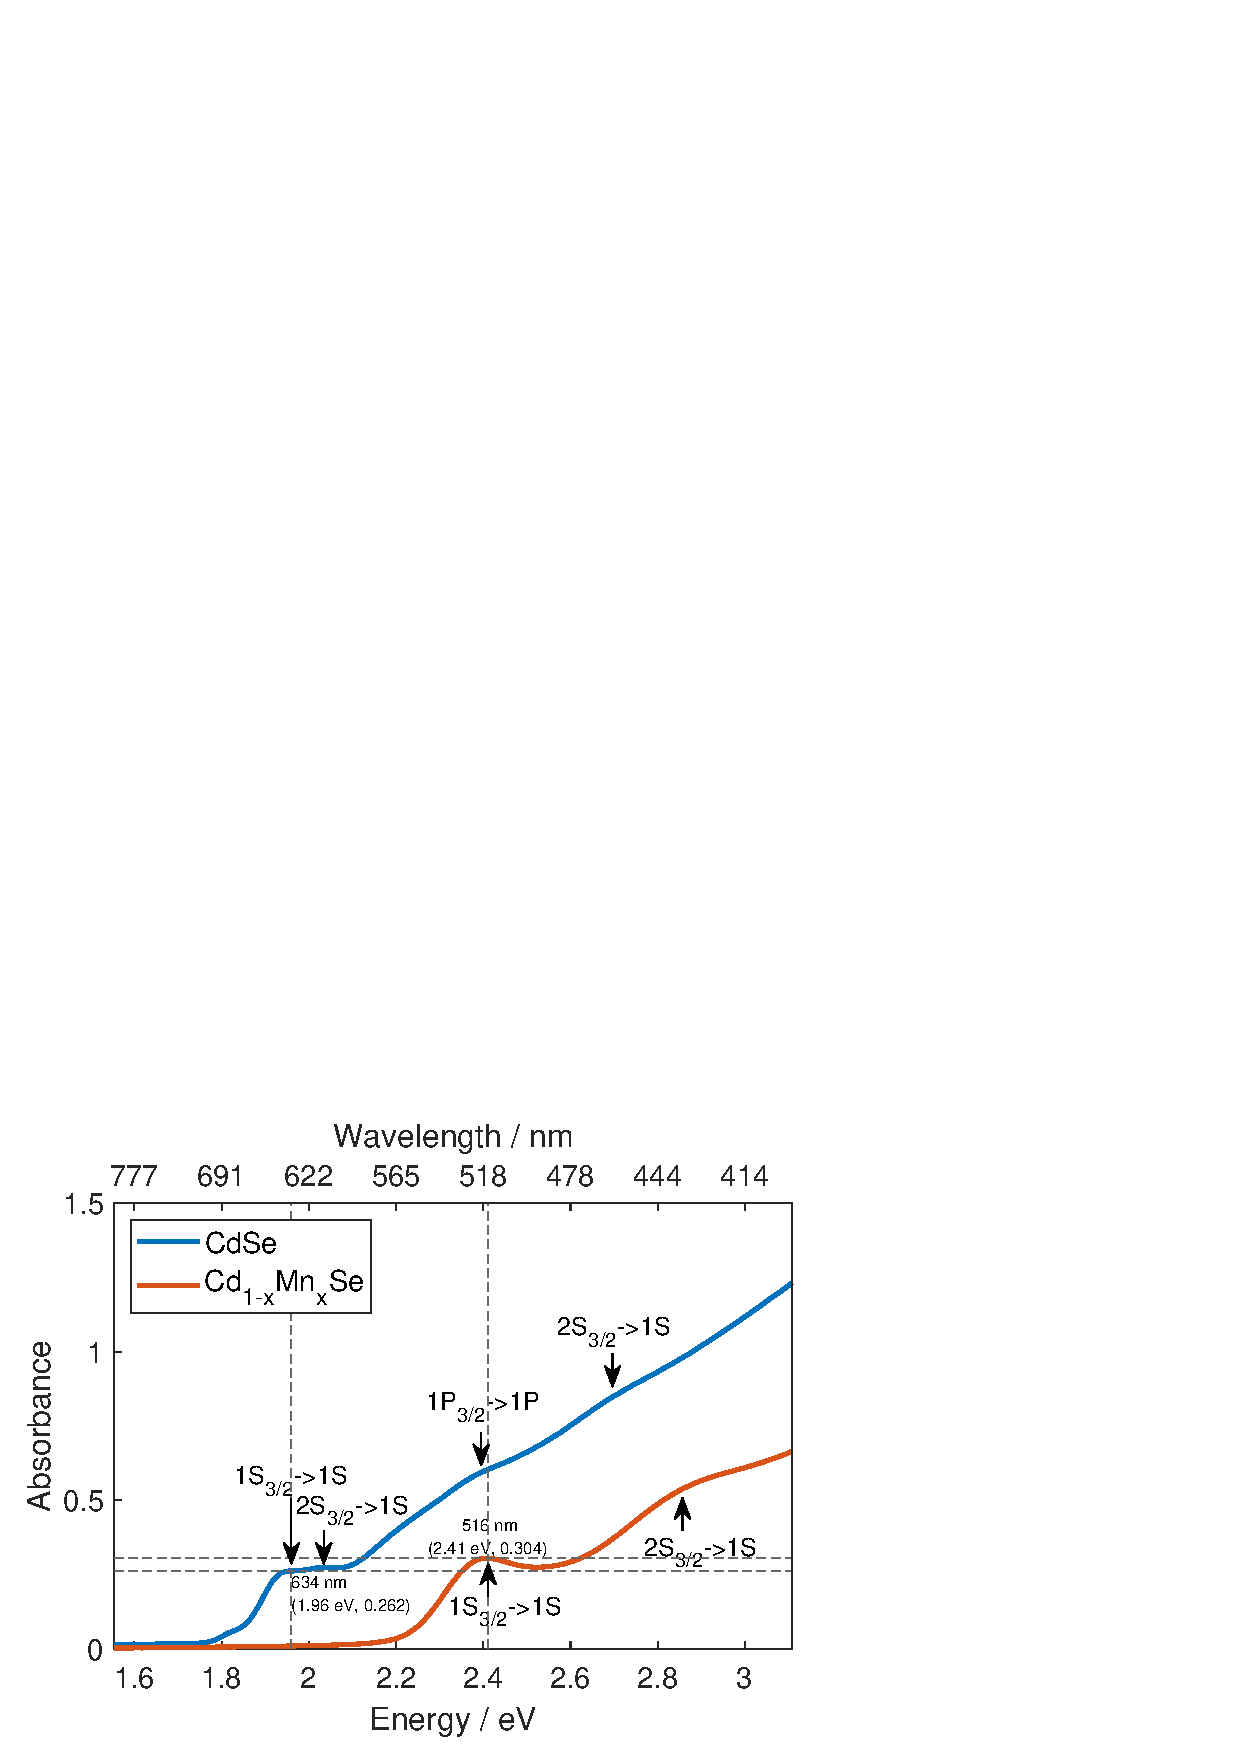
\includegraphics[width=.8\columnwidth]{Quantum-Dot-CdSe-and-Cd1-xMnxSe-Absorption-Spectrum.pdf}
    \caption{(a)(b) \ce{CdSe} 量子点胶体和 \ce{Cd_{1-x}Mn_xSe} 量子点胶体的吸收谱及其二阶导数,其中竖直虚线标注了吸收谱二阶导数的极小值点及其对应的激子能级。}
    \label{Absorption spectrum}
\end{figure}

\ce{CdSe} 量子点的 1S$_{3/2}\rightarrow$1(e) 跃迁的能量为 $1.92$ eV,对应波长为 $646$ nm。根据经验公式\cite{jasieniak2009re}
\begin{align}
    \notag D(\text{nm})=&59.60816-0.54736[\lambda(\text{nm})]+1.8873\times 10^{-3}[\lambda(\text{nm})]^2-2.85743\times 10^{-6}[\lambda(\text{nm})]^3\\
    &+1.62974\times 10^{-9}[\lambda(\text{nm})]^4,
\end{align}
量子点的直径约为 $7.11$ nm。我们还尝试着使用布鲁斯公式估算了量子点的直径。对于闪锌矿型的体块 \ce{CdSe},带隙为 $1.74$ eV\cite{ninomiya1995optical,janowitz1994dielectric},电子和(重)空穴的有效质量分别为 $m_e^*=0.12 m_e$ 和 $m_h^*=0.9 m_e$($100$ 方向;其中 $m_e$ 为电子质量)\cite{kim1994optical},在波长为 $627.2$ nm (对应光子能量为 $1.982$ eV)的光下的相对介电常数 $\epsilon_r=8.0251$\cite{reshak2006theoretical},我们利用布鲁斯公式(式 \eqref{Brus Equ})计算得到 \ce{CdSe} 量子点的直径为 $7.21$ nm,与上面经验公式的计算结果相近。

\ce{CdSe} 量子点在 $686$ nm 处有一较小的吸收峰,这并非 \ce{CdSe} 量子点的典型吸收谱的特征,据推测是对应样品中的少部分尺寸较大的量子点的 1S$_{32}\rightarrow$1S(e) 跃迁。

\section{实验装置}
如图 \eqref{2D Spectrum System} 展示了本实验的装置:我们利用飞秒激光器(图 \ref{2D Spectrum System} \textcircled{\footnotesize{1}})作为激光源,产生重复频率为 $100$ kHz,波长为 $1030$ nm 的激光脉冲,输出总功率为 $40.000$ W,故每个激光脉冲携带有 $400$ $\mu$J 的能量。每个激光脉冲由半透半反镜分为两束,一束经过光参量放大器(optical parametric amplifier,简称 OPA,图 \ref{2D Spectrum System} \textcircled{\footnotesize{4}})转换为 $1280$ nm 波长后,通过厚度为 $1$ mm 的硼酸钡(barium borate,化学式 \ce{Ba(BO2)2},简称 BBO,图 \ref{2D Spectrum System} \textcircled{\footnotesize{5}})晶体,利用 BBO 晶体的二次谐波产生(second harmonic generation,简称 SHG)效应转换为 $640$ nm 波长,将其输入脉冲整形器(pulse shaper,图 \ref{2D Spectrum System} I),从而使单个脉冲重整为时间间隔可以调节的两个相邻脉冲,作为泵浦光(pump beam)照射样品(图 \ref{2D Spectrum System} \textcircled{\footnotesize{11}});另一路激光脉冲经过置于水平位移台(图 \textcircled{\footnotesize{11}})上的一对反射镜的反射,得到相对于泵浦脉冲的时延,再经一钇铝石榴石(yttrium aluminium garnet,化学式 \ce{Y3Al5O12},简称 YAG)晶体通过非线性效应产生主要能量集中于 $540$ nm 至 $700$ nm 波段范围内的白光,作为探测光(probe beam)输入样品。探测光与泵浦光的光路交汇于样品的同一点,但探测光相对于泵浦光存在时延。在探测光传播方向上的单色仪(monochrometer,图 \ref{2D Spectrum System} 左侧圆角矩形)将信号光在水平面上按照波长展开,用高速线扫描相机(图 \ref{2D Spectrum System} \textcircled{\footnotesize{11}})对各波长的信号进行采样。

\begin{figure}[h!]
    \centering
    \includegraphics[width=1\columnwidth]{Img/2D Spectrum System.png}
    \caption{二维光谱系统. \textcircled{\footnotesize{1}} --- 激光源(Light Conversion Inc, CARBIDE - CB3),\textcircled{\footnotesize{2}} --- 平面反射镜,\textcircled{\footnotesize{3}} --- 半透半反镜,\textcircled{\footnotesize{4}} --- 光参量放大器(Light Conversion, ORPHEUS-TWINS),\textcircled{\footnotesize{5}} --- BBO 晶体,\textcircled{\footnotesize{6}} --- 水平位移台(Thorlabs, LTS300),\textcircled{\footnotesize{7}} --- 反射光栅,\textcircled{\footnotesize{8}} --- 离轴抛物柱面反射镜,\textcircled{\footnotesize{9}} --- 声光调制器,\textcircled{\footnotesize{10}} --- 非线性晶体,\textcircled{\footnotesize{11}} --- 样品,\textcircled{\footnotesize{12}} --- 线扫描相机(Teledyne e2v 公司, OCTOPLUS BA2),I --- 脉冲整形器(PhaseTech 公司, QuickShape Visible),II --- 光栅光谱仪(其中单色仪为北京卓立汉光仪器有限公司的 Omni-$\lambda$200i 系列)。}
    \label{2D Spectrum System}
\end{figure}

如图 \ref{2D Spectrum System}(a) 中所示,在脉冲整形器中,反射光栅将每个脉冲中不同波长的成分以不同角度反射,再由焦点位于反射光栅处的离轴抛物柱面反射镜反射而转换为平行光,从而实现对脉冲中不同波长的成分在空间上的分离。脉冲整形器的高速任意波发生器(arbitrary wave generator,简称 AWG)将脉冲整形所需的掩模函数转换为含时射频信号,这一信号经过放大后驱动声光调制器(acousto-optic modulator,简称 AOM)中的压电换能器(piezoelctric transducer)以在 AOM 的 \ce{TiO2} 晶体中产生声波(密度疏密的空间分布),从而引起其折射率的空间分布,激光脉冲穿过这一特殊的“光栅”时就等效于对激光脉冲在频域进行调制。完成调制的激光脉冲再经过另一组对称的离轴抛物柱面反射镜和反射光栅的逆操作,即可在空间上重新合并为一束。在适合的信号激励下,可以将脉冲调制为所需的波形。

脉冲整形器有两种模式,一种是 chop on-chop off 模式,另一种是 phase cycling 模式。在 chop on-chop off 模式下,可以控制输入脉冲依次通过和不通过脉冲整形器,这一模式可以用于瞬态吸收谱的测量。在 phase cycling 模式下,每个输入的脉冲被一分为二,输出的两个脉冲之间的时延可调,并且两个脉冲带有给定的相位,通过调节 AOM 的射频功率还可以控制脉冲的强度,这一模式可以用于二维光谱的测量。

% 我们通过改变 AOM 的折射率分布可以调节产生的每一对泵浦脉冲中两个脉冲间的时延 $\tau$。

% 实际实验中,由于线扫描相机在对奇数行和偶数行采样时分别使用两组不同的像素点,为了避免使用不同的像素点而引入的误差,我们以 $4$ 对泵浦脉冲为一组,分别施加 $0$, $0$, $\pi$, $\pi$ 的相位,并且只取采样得到的奇数或偶数行的信号进行分析。

扫描泵浦脉冲间的时延 $\tau$ 并关于 $\tau$ 作傅里叶变换,得到的泵浦频率即为所谓二维光谱的其中一维。而探测光的频率则构成了二维光谱的另一维。由单色仪和线扫描相机组装而成了光栅光谱仪,当探测光和信号光一同进入单色仪后,经一平面反射镜和离轴抛物柱面反射镜准直,被一反射光栅分光,使不同波长的成分在空间上分开,再经另一组离轴抛物柱面反射镜和平面反射镜汇聚于线扫描相机,经过换算可以将线扫描相机的像素点与光波长对应起来,从而得到光谱。

此外,通过调节水平位移台的前后移动,还可以改变探测光相对于泵浦光的时延 $T$,从而能够研究激发态的弛豫过程的快慢。

在利用二维光谱系统对样品进行测量时,我们将 \ce{CdSe} 量子点胶体装于厚度为 $1.00$ mm 的石英比色皿(图 \ref{2D Spectrum System} \textcircled{\footnotesize{11}})中。

\section{瞬态吸收谱}
当泵浦光强度很大时,可能发生一个量子点在单个泵浦脉冲激发下吸收超过一个光子,即多激子激发的情形(multi-exciton regime)。为了抑制多激子激发而保证单光子激发的情形主导,我们需要泵浦光的强度低于某一阈值,而为了得到尽可能高的信噪比,我们又需要泵浦光的强度尽可能强。为此,我们需要确定一个最适宜的泵浦功率。

我们首先估算了单个量子点在每个脉冲中吸收的光子数。根据经验公式\cite{jasieniak2009re}
\begin{align}
    \varepsilon_{\text{1S}_{3/2}\text{(h)}\rightarrow\text{1S(e)}}(\text{mol}^{-1}\text{cm}^{-1})=155507+6.67054\times 10^{13}\exp\left(-\frac{E_{\text{1S}_{3/2}\rightarrow\text{1S(e)}}}{0.10551}\right),
\end{align}
计算得到 \ce{CdSe} 量子点胶体的 1S$_{3/2}\rightarrow$1S(e) 跃迁贡献的摩尔消光系数为 $9.56\times 10^5\text{mol}^{-1}$。摩尔消光系数和散射截面存在关系\cite{jasieniak2009re}
\begin{align}
    \varepsilon=\frac{N_A\times\sigma}{1000\times\ln(10)}
\end{align}
其中 $N_A$ 为阿伏伽德罗常数,故换算得到单颗 \ce{CdSe} 量子点的散射截面为 $\sigma=3.66\times 10^{-15}$ cm$^2$。

在 AOM 射频功率为 $20\%$ 的情况下,我们用功率计测量了通过直径为 $50$ $\mu$m 的针孔光阑的泵浦光的功率约为 $50$ $\mu$W,故每个泵浦脉冲的单位截面上的能量密度为 $1.27$ J/cm$^2$,单位截面上通过的光子数为 $4.10\times 10^{13}$ cm$^{-2}$,故平均每颗量子点吸收 $N=0.150$ 个光子。若将量子点吸收光子的过程建模为泊松过程,则单颗量子点在与每个泵浦脉冲相互作用时吸收 $n$ 个光子的概率为
\begin{align}
    P(n)=\frac{N^n}{n!}\exp(-N).
\end{align}
由上式得到单个量子点在与每个泵浦脉冲相互作用时吸收单个光子的概率为 $12.9\%$,远高于吸收两个光子的概率($1.0\%$),因此 AOM 射频功率为 $20\%$ 时泵浦光的强度应当可以保证单激子激发情形。

为了确保泵浦光与量子点胶体的相互作用是以单激子激发情形主导的,我们还测量了瞬态吸收谱。图 \ref{Transient Absorption}(a) 展示了瞬态吸收实验的脉冲序列的设定,脉冲整形器工作在 chop on-chop off 模式,并且扫描泵浦脉冲和探测脉冲间的时延 $T$,由于线扫描相机在对奇数行和偶数行采样时分别使用两组不同的像素点,因此每个脉冲序列重复两遍,奇数行和偶数行分别处理。将有泵浦时的探测光透射强度与无泵浦时的探测光透射强度相减并处以无泵浦时的探测光强度,得到的探测光透射强度变化率即为瞬态吸收谱。扫描 AOM 射频功率,得到不同泵浦强度下,泵浦-探测时延 $T=1.8$ ps 时,在 $646$ nm 波长处的透射强度变化率,如图 \ref{Transient Absorption}(b) 所示。当 AOM 射频功率在 $15\%$ 以下时,瞬态吸收强度关于 AOM 射频功率呈现较好的线性递增关系,而当 AOM 射频功率超过 $15\%$ 后,瞬态吸收随 AOM 射频功率的增长逐渐放缓,偏离了线性关系。这说明,AOM 射频功率在 $15\%$ 以下时,样品处于单激子激发的情形。

\begin{figure}[h]
    \centering
    \includegraphics[width=1\columnwidth]{Img/Transient Absorption.pdf}
    \caption{瞬态吸收。(a) 瞬态吸收实验的脉冲序列:chop on-chop off 模式,并且扫描泵浦-脉冲时延,每种序列重复两遍。(b) $T=1.8$ ps,$646$ nm 波长透射强度改变量关于 AOM 射频功率的变化关系。(c) AOM 射频功率为 $10\%$ 时测得的瞬态吸收谱。(d) 不同泵浦-探测时延下的瞬态吸收谱,虚线是用于对照的 \ce{CdSe} 的吸收谱。(e) $646$ nm, $622$ nm, $592$ nm 和 $540$ nm 波长的透射强度关于泵浦-探测时延的变化。}
    \label{Transient Absorption}
\end{figure}

这里我们设定 AOM 射频功率为 $10\%$,测得如图 \ref{Transient Absorption} 所示的瞬态吸收谱。由于探测光的强度主要集中于 $540$ nm 至 $700$ nm 波长范围内,瞬态吸收谱中该波长范围以外的区域信噪比较差。在 $540$ nm 至 $700$ nm 波长范围内,除了由于泵浦光对 1S$_{3/2}\rightarrow$1S(e) 跃迁的漂白效应导致的 $646$ nm 波长处的透射增强,还有在 $620$ nm 波长附近的透射增强和 $590$ nm 波长附近的透射减弱,这两个特征均在泵浦后皮秒量级的时间内出现。$646$ nm 处的透射强度改变量随泵浦-探测时延呈现较明显的波动,可能是来源于激光输出功率的波动。

图 \ref{Transient Absorption}(d) 分别截取了泵浦-探测时延 $T$ 为 $1$ ps, $10$ ps, $100$ ps 的透射谱。$T=1$ ps 波长 $646$ nm 处透射强度小于 $T=10$ ps 的透射强度信号,这主要是因为实验中缺少对泵浦脉冲的色散补偿,泵浦脉冲在时域上的宽度较大,这导致部分泵浦脉冲的一小部分在 $T=1$ ps 之后到达样品,因此在 $T=1$ ps 时泵浦光对 1S$_{3/2}\rightarrow$1S(e) 跃迁的漂白效果尚未达到最大。$T=100$ ps $646$ nm 处的透射强度相对于 $T=10$ ps 有所衰减,这来源于 $\lvert 1\rangle$ 态激子的复合。$620$ nm 附近的透射增强对应于 2S$_{1/2}\rightarrow$1S(e) 跃迁,由于激子间的耦合,$620$ nm 略小于 2S$_{1/2}\rightarrow$1S(e) 跃迁的 $613$ nm,泵浦脉冲的激发增加了 1S(e) 的布居,从而抑制了 2S$_{1/2}\rightarrow$1S(e) 跃迁。

图 \ref{Transient Absorption}(e) 分别追踪了 $646$ nm, $622$ nm, $592$ nm 和 $540$ nm 波长的透射强度关于泵浦-探测时延的变化。多激子激发的情形往往伴随着明显的俄歇复合,特征时间在皮秒量级,而图中这些特征在 $500$ ps 的时延范围内,均无显著的衰减,这说明目前的泵浦脉冲强度下,系统的激发属于单激子激发情形。

\section{二维光谱}
设定 AOM 射频功率为 $10\%$,采用如图 \ref{2D Spectrum}(a) 所示的脉冲序列,对于每个给定的泵浦间脉冲 $\tau$,分别对两个泵浦施加 $(0,0)$, $(\pi,0)$, $(\pi,\pi)$ 和 $(0,\pi)$,得到信号 $S(0,0)$, $S(\pi,0)$, $S(\pi,\pi)$ 和 $S(0,\pi)$,通过运算 $S(0,0)-S(\pi,0)+S(\pi,\pi)-S(0,\pi)$ 将瞬态吸收信号去除;对于给定的泵浦-探测时延 $T$,将探测脉冲移至第一个泵浦脉冲前 $T$ 处重复实验(图中未画出),将正的泵浦-探测时延下得到的信号与负的泵浦-探测时延下得到的信号相减以去除泵浦光的散射导致的噪声。在 $T=1$ ps, $10$ ps 和 $100$ ps 的情况下,得到了如图 \ref{2D Spectrum}(b)-(d) 所示的二维光谱。由于泵浦光的绝大部分能量集中于 \ce{CdSe} 量子点的 1S$_{3/2}\rightarrow$1S(e) 跃迁能量附近,因此二维光谱中仅在泵浦能量为 \ce{CdSe} 量子点的 1S$_{3/2}\rightarrow$1S(e) 跃迁能量处有信号峰,信号峰的探测能量分别对应着探测光引发的跃迁能量。其中,对角线上的信号峰反应了泵浦光对 1S$_{3/2}\rightarrow$1S(e) 的漂白效果,以及 1S$_{3/2}$ 向 1S(e) 的受激辐射。非对角峰与前一节所述同理,对应着 1S$_{3/2}\rightarrow$1S(e) 跃迁与 2S$_{1/2}\rightarrow$1S(e) 等跃迁之间的耦合。

在 $100$ ps 的泵浦间时延范围内,信号没有明显的衰减,并且信号峰的探测能量和信号峰的正负也与上一节中瞬态吸收谱的信号峰非常相似。实际上,真正的二维光谱信号应该在(最多)皮秒量级就已经充分衰减,图中所示的能够持续百皮秒量级的信号大部分是瞬态吸收的贡献。由于实验中没有对泵浦脉冲的色散补偿,泵浦脉冲在时域上的宽度较大,两个泵浦脉冲时间存在部分的交叠,从而相互干涉,当扫描 $\tau$,干涉得到的泵浦脉冲的总强度周期性变化,从而贡献了图中的泵浦频率为泵浦脉冲中心频率的信号峰。

\begin{figure}[h]
    \centering
    \includegraphics[width=1\columnwidth]{Img/2D Spectrum.pdf}
    \caption{二维光谱。(a) 二维光谱实验的脉冲序列。(b)-(d) 泵浦-探测时延分别在 $T=1$ ps, $10$ ps, $100$ ps 时得到的二维光谱。(e) 对泵浦-探测时延分别在 $T=1$ ps, $10$ ps, $100$ ps 时得到的二维光谱关于泵浦能量积分得到的结果,虚线是用于对照的 \ce{CdSe} 的吸收谱。}
    \label{2D Spectrum}
\end{figure}

图 \ref{2D Spectrum}(e) 是将信号关于泵浦能量积分所得,与 \ref{Transient Absorption}(d) 中的瞬态吸收谱相近,未能明显看出其中二维光谱信号的衰减,这也佐证了我们的信号很大一部分来源于瞬态吸收过程的贡献的说法。

作为对照,我们还换用 \ce{Cd_{1-x}Mn_xSe} 进行了同样的测量,得到了不同的信号峰分布(图略),由此可以证明上述信号是和样品的能级结构有关的,而非人为引入的误差或仪器缺陷导致的错误信号。

\chapter{结论和展望}
我们首先利用硒化镉量子点紫外可见吸收光谱的二阶导数,确定了硒化镉量子点低能量处的几个激子能级 --- 1S$_{3/2}\rightarrow$1S(e)、2S$_{3/2}\rightarrow$1S(e)、1P$_{3/2}\rightarrow$1P(e) 和 2S$_{1/2}\rightarrow$1S(e),然后通过瞬态吸收谱确定了产生单激子激发的泵浦能量范围,并且观察到了激子的弛豫,以及 1S$_{3/2}\rightarrow$1S(e) 跃迁和 2S$_{3/2}\rightarrow$1S(e) 等跃迁之间的耦合。在确保单激子激发的前提下,我们测量了硒化镉量子点的二维光谱,由于未对泵浦脉冲进行色散补偿,瞬态吸收过程在二维光谱信号峰处产生了较为显著的贡献,其信号掩盖了真正的二维光谱信号,因此我们的二维光谱中信号峰的强度在皮秒量级的泵浦-探测时延下并无显著的衰减。后续,可以对泵浦脉冲进行色散补偿,从而提升二维光谱的信号质量。

\chapter{附录}
\section{刘维尔 - 冯诺依曼方程与双边费曼图}
\subsection{刘维尔 - 冯诺依曼方程的证明}
刘维尔 - 冯诺依曼方程是用于描述系统的密度矩阵随时间的演化的偏微分方程,可以由用于描述系统的量子态随时间演化的薛定谔方程推导得到。假设某系统在 $t$ 时刻的密度矩阵为
\begin{align}
    \hat{\rho}(t)=\sum_nP_n\lvert\psi_n(t)\rangle\langle\psi_n(t)\rvert,
\end{align}
其中某一纯态 $\lvert\psi_n(t)\rangle$ 随时间的演化遵循薛定谔方程,
\begin{align}
    \label{Shrodinger-Equ}
    \frac{\partial}{\partial t}\lvert\psi_n(t)\rangle=-\frac{i}{\hbar}\hat{H}\lvert\psi_n(t)\rangle,
\end{align}
其中 $\hat{H}(t)$ 为系统的哈密顿量,
则系统的密度矩阵随时间的演化遵循
\begin{align}
    \notag\frac{\partial}{\partial t}\hat{\rho}(t)=&\frac{\partial}{\partial t}\sum_nP_n\lvert\psi_n(t)\rangle\langle\psi_n(t)\rvert\\
    =&\sum_nP_n\left[\left(\frac{\partial}{\partial t}\lvert\psi_n(t)\rangle\right)\langle\psi_n(t)\rvert+\lvert\psi_n(t)\rangle\left(\frac{\partial}{\partial t}\lvert\psi_n(t)\rangle\right)^{\dagger}\right].
\end{align}
根据薛定谔方程(式 \eqref{Shrodinger-Equ}),用 $-\frac{i}{\hbar}\hat{H}$ 代替上式中的 $\frac{\partial}{\partial t}$,有
\begin{align}
    \notag\frac{\partial}{\partial t}\hat{\rho}(t)=&\sum_nP_n\left[-\frac{i}{\hbar}\hat{H}\lvert\psi_n(t)\rangle\langle\psi_n(t)\rvert+\lvert\psi_n(t)\rangle\left(-\frac{i}{\hbar}\hat{H}\lvert\psi_n(t)\rangle\right)^{\dagger}\right]\\
    \notag=&\sum_nP_n\left[-\frac{i}{\hbar}\hat{H}\lvert\psi_n(t)\rangle\langle\psi_n(t)\rvert+\frac{i}{\hbar}\lvert\psi_n(t)\rangle\langle\psi_n(t)\rvert\hat{H}\right]\\
    \notag=&-\frac{i}{\hbar}\left[\hat{H}\sum_nP_n\lvert\psi_i(t)\rangle\langle\psi_i(t)\rvert-\sum_nP_n\lvert\psi_n(t)\rangle\langle\psi_n(t)\rvert\hat{H}\right]\\
    =&-\frac{i}{\hbar}\left[\hat{H}\hat{\rho}(t)-\hat{\rho}(t)\hat{H}\right],
\end{align}
\begin{gather}
    \label{von Neumann Equ}
    \Longrightarrow i\hbar\frac{\partial}{\partial t}\hat{\rho}=[\hat{H},\hat{\rho}(t)].
\end{gather}
此即\textbf{刘维尔 - 冯诺依曼方程},其中 $[\cdots]$ 代表对易子,即 $[\hat{H},\hat{\rho}]=\hat{H}\hat{\rho}-\hat{\rho}\hat{H}$.

\subsection{刘维尔 - 冯诺依曼方程的求解}
\label{von Neumann Equ sol}
上一小节中所列的为冯诺依曼方程在薛定谔绘景(Schrödinger Picture)中的形式。当系统的哈密顿量与时间有关,即系统的总哈密顿量可以表示为不含时的无微扰哈密顿量 $H_0$ 与含时的微扰哈密顿量 $\hat{H}_I(t)$ 之和,
\begin{align}
    \hat{H}(t)=\hat{H}_0+\hat{H}_I(t),
\end{align}
上述形式的冯诺依曼方程并不容易求解。为了便于求解冯诺依曼方程,我们首先需要暂时将其由薛定谔绘景转入相互作用绘景(Interaction Picture,又称狄拉克绘景,Dirac Picture),利用微扰理论求解得到相互作用绘景中的密度矩阵后,再将其转化回薛定谔绘景中。
在相互作用绘景中,任一可观测物理量 $O$ 的算符表示为
\begin{align}
    \hat{O}'(t)=\hat{U}_0(-t)\hat{O}(t)\hat{U}_0(t),
\end{align}
其中 $\hat{O}(t)$ 为可观测物理量 $O$ 的算符在薛定谔绘景中的形式,不含时无微扰哈密顿量对应的时间演化算符 $\hat{U}_0(t)=\exp\left[-\frac{i}{\hbar}\int_0^t\hat{H}_0\,\mathrm{d}\tau\right]$。
在相互作用绘景中,系统密度矩阵也可以用相似的方式表示为
\begin{align}
    \hat{\rho}'(t)=\hat{U}_0(-t)\hat{\rho}(t)\hat{U}_0(t).
\end{align}
其关于时间的演化遵循
\begin{align}
    \frac{\partial}{\partial t}\hat{\rho}'(t)=\left[\frac{\partial}{\partial t}\hat{U}_0(-t)\right]\hat{\rho}(t)\hat{U}_0(t)+\hat{U}_0(-t)\left[\frac{\partial}{\partial t}\hat{\rho}(t)\right]\hat{U}_0(t)+\hat{U}_0(-t)\hat{\rho}(t)\left[\frac{\partial}{\partial t}\hat{U}_0(t)\right],
\end{align}
其中
\begin{align}
    \notag\frac{\partial}{\partial t}\hat{U}_0(t)=&\frac{\partial}{\partial t}\exp\left[-\frac{i}{\hbar}\hat{H}_0t\right]=\frac{\partial}{\partial t}\sum_{n=0}^{\infty}\frac{1}{n!}\left[-\frac{i}{\hbar}\hat{H}_0t\right]^n=\sum_{n=1}^{\infty}\frac{1}{(n-1)!}\left[-\frac{i}{\hbar}\hat{H}_0\right]^nt^{n-1}\\
    =&-\frac{i}{\hbar}\hat{H}_0\sum_{n=0}\frac{1}{n!}\left[-\frac{i}{\hbar}\hat{H}_0t\right]^n=-\frac{i}{\hbar}\hat{H}_0\exp\left[-\frac{i}{\hbar}\hat{H}_0t\right]=-\frac{i}{\hbar}\hat{H}_0\hat{U}_0(t),
\end{align}
而
\begin{align}
    \frac{\partial}{\partial t}\hat{U}_0(-t)=-\frac{\partial}{\partial(-t)}\hat{U}_0(-t)=\frac{i}{\hbar}\hat{H}_0\hat{U}_0(-t),
\end{align}
以及根据刘维尔方程(式 \eqref{von Neumann Equ}),故有
\begin{align}
    \label{Density matrix evolution in interaction pic}
    \frac{\partial}{\partial t}\hat{\rho}'(t)=\frac{i}{\hbar}\hat{H}_0\hat{U}_0(-t)\hat{\rho}(t)\hat{U}_0(t)-\frac{i}{\hbar}\hat{U}_0(t)[\hat{H}_0(t)+\hat{H}_I(t),\hat{\rho}(t)]\hat{U}_0(t)-\frac{i}{\hbar}\hat{U}_0(-t)\hat{\rho}(t)\hat{H}_0\hat{U}_0(t).
\end{align}
由于 $\hat{U}_0(t)$ 可以展开为关于 $\hat{H}_0$ 的多项式,故 $\hat{U}_0(t)$ 与 $\hat{H}_0$ 对易,
\begin{align}
    \notag[\hat{U}_0(t),\hat{H}_0]=&\hat{U}_0\hat{H}_0-\hat{H}_0\hat{U}_0(t)=\exp\left[-\frac{i}{\hbar}\hat{H}_0t\right]\hat{H}_0-\hat{H}_0\exp\left[-\frac{i}{\hbar}\hat{H}_0t\right]\\
    =&\sum_{n=0}^{\infty}\frac{1}{n!}\left(-\frac{i}{\hbar}\hat{H}_0t\right)^n\hat{H}_0-\hat{H}_0\sum_{n=0}^{\infty}\frac{1}{n!}\left(-\frac{i}{\hbar}H_0t\right)^n=0.
\end{align}
因此式 \eqref{Density matrix evolution in interaction pic} 可以进一步化为
\begin{align}
    \notag\frac{\partial}{\partial t}\hat{\rho}'(t)=&\frac{i}{\hbar}\hat{H}_0\hat{U}_0(-t)\hat{\rho}(t)\hat{U}_0(t)-\frac{i}{\hbar}\hat{H}_0\hat{U}_0(-t)\hat{\rho}(t)\hat{U}_0(t)+\frac{i}{\hbar}\hat{U}_0(-t)\hat{\rho}(t)\hat{U}_0(t)\hat{H}_0\\
    \notag&-\frac{i}{\hbar}\hat{U}_0(-t)[\hat{H}_I(t),\hat{\rho}(t)]\hat{U}_0(t)-\frac{i}{\hbar}\hat{U}_0(-t)\hat{\rho}(t)\hat{U}_0(t)\hat{H}_0\\
    =&-\frac{i}{\hbar}\hat{U}_0(-t)[\hat{H}_I(t),\hat{\rho}(t)]\hat{U}_0(t).
\end{align}
向上式中插入单位算符 $\hat{1}=\hat{U}_0(t)\hat{U}_0(-t)$,可以将式中的微扰哈密顿量 $\hat{H}_I$ 和密度矩阵 $\hat{\rho}$ 均转化为相互作用表象中的形式,
\begin{align}
    \notag\frac{\partial}{\partial t}\hat{\rho}'(t)=&-\frac{i}{\hbar}\hat{U}_0(-t)\hat{H}_I(t)\hat{1}\hat{\rho}(t)\hat{U}_0(t)+\frac{i}{\hbar}\hat{U}_0(-t)\hat{\rho}(t)\hat{1}\hat{H}_I(t)\hat{U}_0(t)\\
    \notag=&-\frac{i}{\hbar}\hat{U}_0(-t)\hat{H}_I(t)\hat{U}_0(t)\hat{U}_0(-t)\hat{\rho}(t)\hat{U}_0(t)+\frac{i}{\hbar}\hat{U}_0(-t)\hat{\rho}_0(t)\hat{U}_0(t)\hat{U}_0(-t)\hat{H}_I(t)\hat{U}_0(t)\\
    =&-\frac{i}{\hbar}\hat{H}_I'(t)\hat{\rho}'(t)-\frac{i}{\hbar}\hat{\rho}'(t)\hat{H}_I'(t),
\end{align}
其中 $\hat{H}_I'(t)=\hat{U}_0(-t)\hat{H}_I(t)\hat{U}_0(t)$ 为相互作用绘景中的含时微扰哈密顿量。由此,我们得到相互作用绘景中的冯诺依曼方程为
\begin{align}
    \frac{\partial}{\partial t}\hat{\rho}'(t)=-\frac{i}{\hbar}[\hat{H}_I'(t),\hat{\rho}'(t)].
\end{align}
类似微扰力理论的处理方法,我们引入一个无量纲的系数 $\lambda$,将系统的总哈密顿量改写为
\begin{align}
    \hat{H}(t)=\hat{H}_0+\lambda\hat{H}_I(t).
\end{align}
我们将密度矩阵展开为关于 $\lambda$ 的级数,
\begin{align}
    \hat{\rho}'(t)=\hat{\rho}^{(0)}(t)+\lambda\hat{\rho}^{(1)}(t)+\lambda^2\hat{\rho}^{(2)}(t)+\cdots,
\end{align}
其中 $\hat{\rho}^{(n)}(t)$ 为密度矩阵对微扰的第 $n$ 阶修正项。
将上式代入相互作用绘景中的冯诺依曼方程,
\begin{align}
    \frac{\partial}{\partial t}[\hat{\rho}'^{(0)}(t)+\lambda\hat{\rho}'^{(1)}(t)+\lambda^2\hat{\rho}'^{(2)}(t)+\cdots]=-\frac{i}{\hbar}[\lambda\hat{H}_I'(t),\hat{\rho}'^{(0)}(t)+\lambda\hat{\rho}'^{(1)}(t)+\lambda^2\hat{\rho}'^{(2)}(t)+\cdots],
\end{align}
并对两边同阶级数的系数取等得
\begin{align}
    \frac{\partial}{\partial t}\hat{\rho}'^{(0)}(t)=&0,\\
    \frac{\partial}{\partial t}\hat{\rho}'^{(1)}(t)=&-\frac{i}{\hbar}[\hat{H}_I',\hat{\rho}'^{(0)}(t)],\\
    \notag\cdots&\\
    \frac{\partial}{\partial t}\hat{\rho}'^{(0)}(t)=&-\frac{i}{\hbar}[\hat{H}_I',\hat{\rho}'^{(n-1)}(t)],\\
    \notag\cdots&
\end{align}
对上面各式积分得由密度矩阵低阶修正项推算高阶修正项的递归式,
\begin{align}
    \hat{\rho}'^{(0)}(t)=&\hat{\rho}'^{(0)}(0),\\
    \hat{\rho}'^{(1)}(t)=&-\frac{i}{\hbar}\int_0^t[\hat{H}_I'(t),\hat{\rho}'^{(0)}(t)]\,\mathrm{d}\tau,\\
    \notag\cdots&\\
    \hat{\rho}'^{(n)}(t)=&-\frac{i}{\hbar}\int_0^t[\hat{H}(\tau),\hat{\rho}'^{(n-1)}(\tau)]\,\mathrm{d}\tau,\\
    \notag\cdots&
\end{align}
综合以上各递归式,有
\begin{align}
    \hat{\rho}'^{(0)}(t)=&\hat{\rho}'^{(0)}(0),\\
    \notag\hat{\rho}'^{(n)}(t)=&\left(-\frac{i}{\hbar}\right)^n\int_0^t\mathrm{d}\tau_1\int_0^{\tau_1}\mathrm{d}\tau_2\cdots\int_0^{\tau_{n-1}}\mathrm{d}\tau_{n-1}\,\left[\hat{H}_I'(\tau_1),\left[\hat{H}_I'(\tau_2),\cdots\left[\hat{H}_I'(\tau_n),\hat{\rho}'^{(0)}(\tau_n)\right]\cdots\right]\right]\\
    \notag=&\left(-\frac{i}{\hbar}\right)^n\int_0^t\mathrm{d}\tau_1\int_0^{\tau_1}\mathrm{d}\tau_2\cdots\int_0^{\tau_{n-1}}\mathrm{d}\tau_n\,\left[\hat{H}_I'(\tau_1),\left[\hat{H}_1'(\tau_2),\cdots\left[\hat{H}_I'(\tau_n),\hat{\rho}'^{(0)}(0)\right]\cdots\right]\right],\\
    &\forall n\geq 1.
\end{align}
将密度矩阵由相互作用绘景转化回薛定谔绘景中,得
\begin{align}
    \label{von Neumann Equ sol-1}
    \hat{\rho}^{(0)}(t)=&\hat{U}_0(t)\hat{\rho}'^{(0)}(0)\hat{U}_0(-t),\\
    \label{von Neumann Equ sol-2}
    \notag\hat{\rho}^{(n)}(t)=&\hat{U}_0(t)\hat{\rho}'^{(n)}(t)\hat{U}_0(-t),\\
    \notag=&\left(-\frac{i}{\hbar}\right)^n\hat{U}_0(t)\int_0^t\mathrm{d}\tau_1\int_0^{\tau_1}\mathrm{d}\tau_2\cdots\int_0^{\tau_{n-1}}\mathrm{d}\tau_n\,\times\\
    &\left[\hat{H}_I'(\tau_1),\left[\hat{H}_I'(\tau_2),\cdots\left[\hat{H}_I'(\tau_n),\hat{\rho}^{(0)}(0)\right]\cdots\right]\right]\hat{U}_0(-t),\quad\forall n\geq 1.
\end{align}

\backmatter% initialize the environment
\intotoc{\bibname}% add link to contents table and bookmark
\bibliography{Biblio/ref}% bibliography

\chapter*{致谢}
谢天谢地!这篇论文到这里总算是要画上句号了,然而受了这么多人的帮助,那可得好好说一说。

Here, I should express my appreciation for Professor McGuire in the first place, who is responsible for guiding my senior thesis project. Your help to me does not only begin from this project, but dates back to the spring of 2020 when I take your Non-linear Optics course. It is one of the toughest course I have gone through in my undergraduate years, but also the most useful ones.

紧接着要感谢的必须是梁超逸师兄。在二维光谱的项目中师兄承担了仪器搭建、程序设计、设备维护等一系列困难而繁重的工作,可以说我在该项目上所花的时间精力不及师兄的零头。为了即时得到我们的数据,甚至占用了师兄的非工作时间,甚是抱歉。梁超逸师兄无论在物理原理还是实验技术上都有着超出同龄人的功底,在今后的研究生阶段,梁超逸师兄将是我努力学习的榜样。同时,课题组里的徐小凡、王凯、杜成江等各位师兄都对我的毕业论文给予了无私的帮助,在此一并表示感谢。

此外,当然要没有各位同学和朋友的陪伴和鼓励,那么完成这个课题的体验也将大打折扣。这里要感谢的是和我共同参与二维光谱项目的王晴宇同学以及时常和我聊天的高中同学黄鹏豪,你们缓解了我工作时间的沉闷与压力。

最后,感谢爸爸妈妈。感谢你们一直以来的支持和鼓励。

在将来的真正的科研生涯中,不求顺风顺水,但求能遇到向大家一样优秀而善良的人。

\end{document}